\section{Performance Evaluation}

An Audio Plugin runs in an environment with many other components, sharing CPU resources. Processing of audio data must be completed within discrete time intervals dictated by the audio hardware. Typical audio sampling frequencies are 44.1kHz, 48kHz, 88.2kHz and 96kHz. Using 44.1kHz as an example, this means that all the calculations required for a single sample must be completed within 0,023 ms. Interrupts would be received from the audio hardware at intervals of 0.023ms as well, and this would put too much of a strain on the Operating System of the CPU though. Instead, requests for new audio data are bundled into buffers of samples. The size of the buffers is a parameter that the user can modify, it's usually set at 512 samples, but can be as low as 16 samples.

Increasing the buffer size, increases the amount of time that the CPU has to process audio data. This introduces latency into the system though. A buffer size of 512 samples equates to a latency of 11.60ms. A 16 sample buffer size equates to 0.36ms.

If a single plugin requires 1.0ms to complete its processing then it will not finish in time if the buffer size is set too low. If the buffer size is just high enough, then there still might not be enough CPU resources left for other plugins to complete their tasks.

\subsection{Synchronous Performance}

This project offloads the processing to external SBC devices. However, no resources are saved if the audio plugin is blocked while it waits for the results from the SBC devices. Since the external SBC devices are slower than the main CPU, the processing time will take longer. Adding the time it takes to serialise and deserialise the Datagram packet at each end will degrade performance even more.

Figure~\ref{fig:local_vs_remote} illustrates the problem in more detail.

\begin{figure}[H]
    \centering
    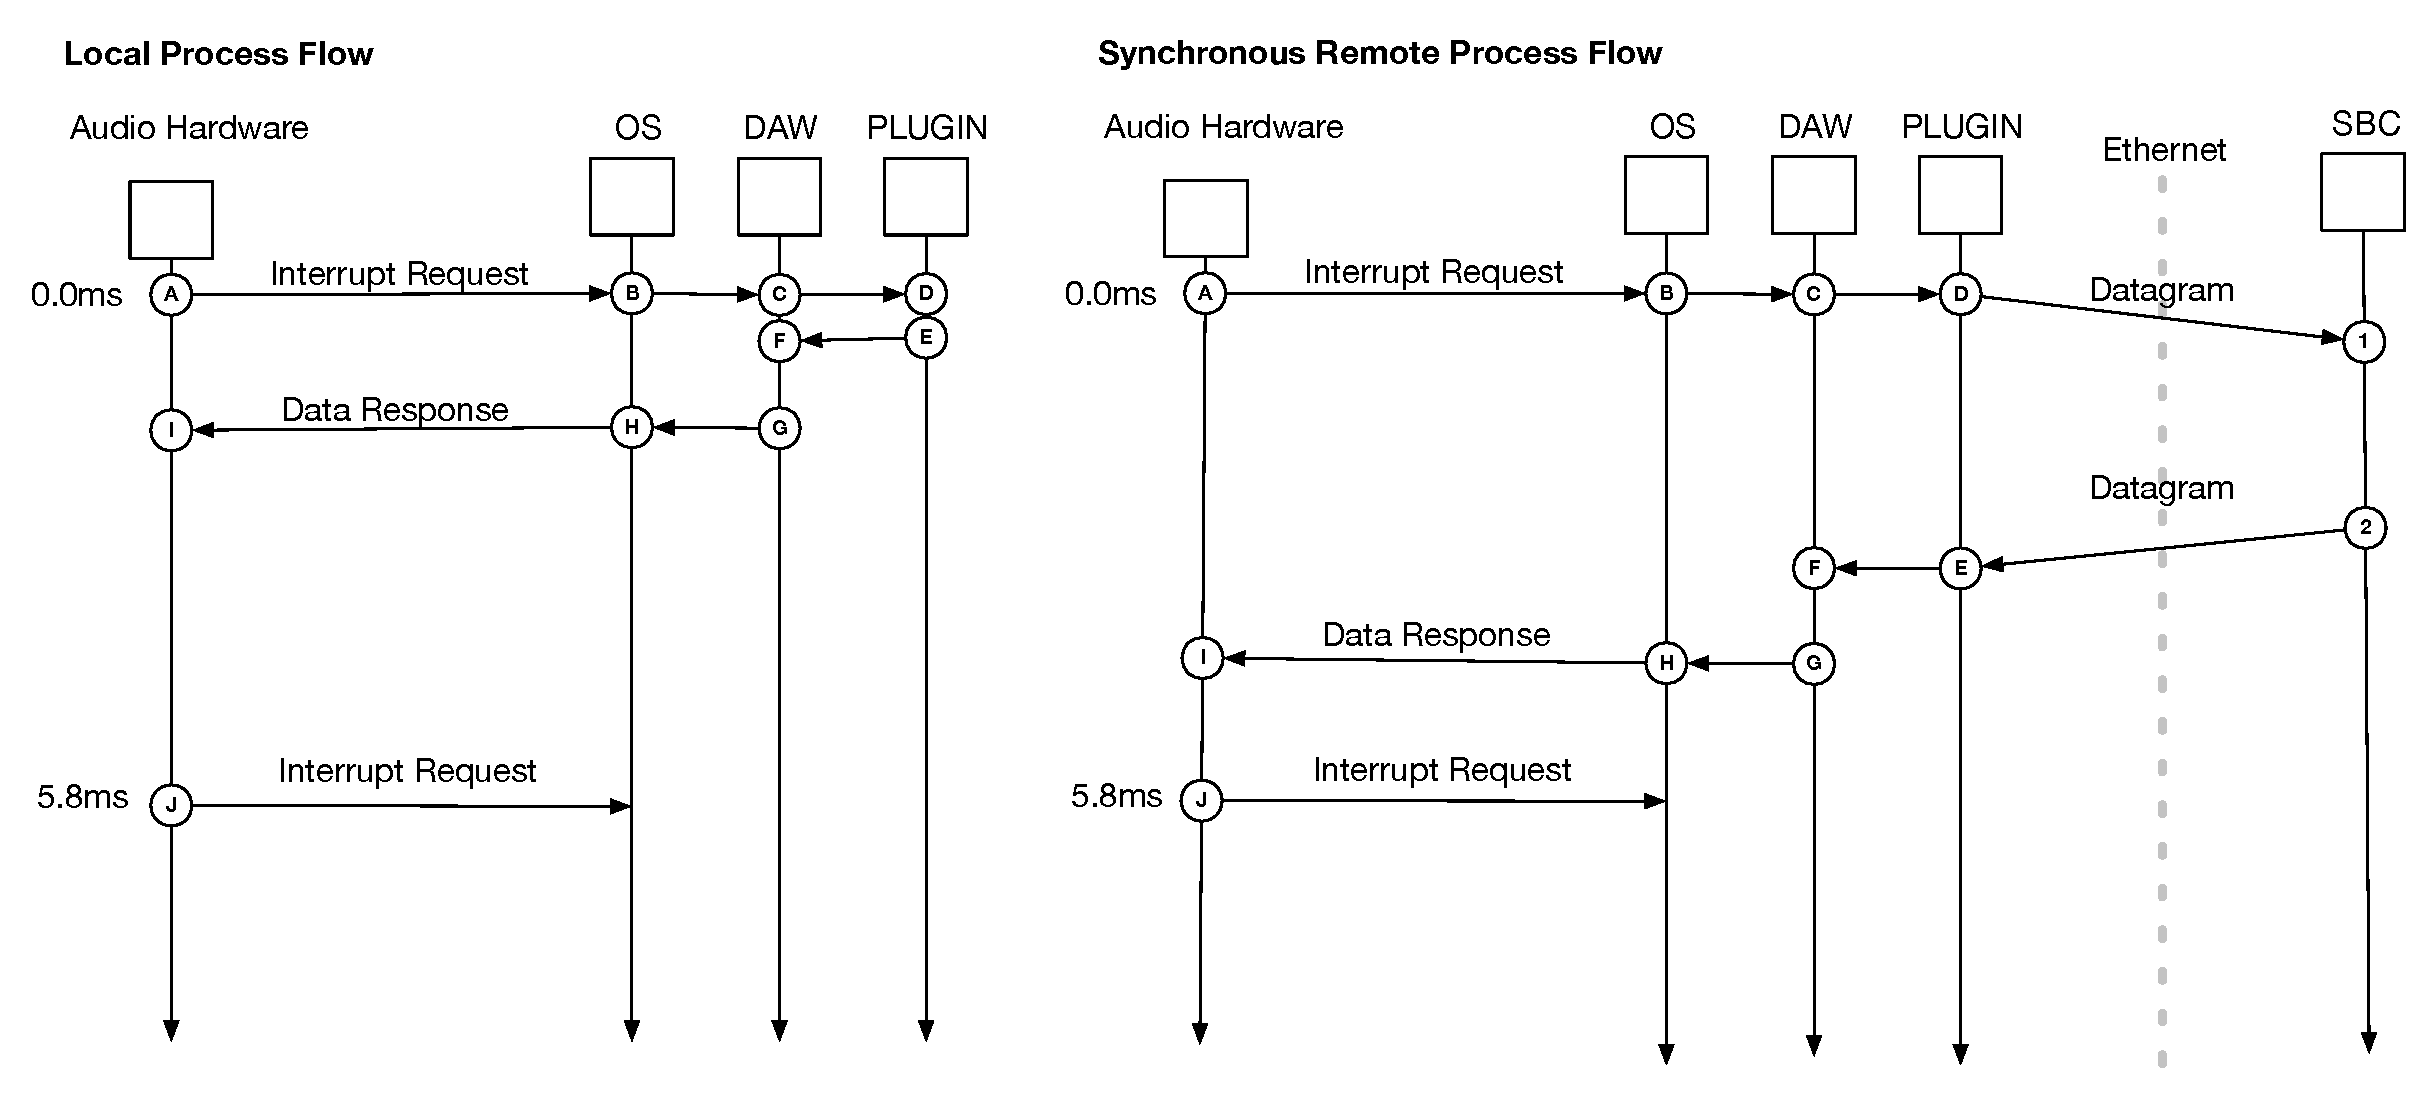
\includegraphics[width=\textwidth]{assets/conclusion/process_flow_compared.pdf}
    \caption{Local vs Remote Synchronous Processing}
    \label{fig:local_vs_remote}
\end{figure}

The example shows the audio hardware polling the operating system in intervals of 5.8 ms. This corresponds to a buffer size of 256 samples. The time interval between states D and E represents the time it takes for a plugin to process a buffer of 256 sample. The DAW  performs other necessary audio processing functions in the interval between F and G. After states G and H the DAW and OS are free to be able to do other things, like update the GUI.

With synchronous remote processing the state E is blocked until states 1 and 2 have completed. If that time is significant then the ability of the DAW and the OS to perform other critical tasks is impaired.

\begin{table}[H]
\begin{center}
\begin{tabular}{ |p{1.4cm}||p{1.5cm}|p{1.7cm}|p{1.7cm}|p{1.6cm}|p{1.4cm}|  }
 \hline
 buffer size    & buffer time (ms)    & rtTime (ms)   & pTime (ms)    & tTime (ms) & \% of buffer time\\
 \hline
 64             & 1.451247      & 0.574672          & 0.015857          & 0.558815      & 39.59 \\
 96             & 2.176870      & 0.575419          & 0.015851          & 0.559568      & 26.43 \\
 128            & 2.902494      & 0.59001           & 0.016519          & 0.573491      & 20.32 \\
 192            & 4.353741      & 0.67902           & 0.019013          & 0.660007      & 15.59 \\
 256            & 5.804988      & 0.707267          & 0.020352          & 0.686915      & 12.18 \\
 512            & 11.60997      & 0.707905          & 0.026348          & 0.681557      & 6.097 \\
 \hline
\end{tabular}
\end{center}
\caption{Measured Times for Synchronous Processing}
\label{tab:latency_comp}
\end{table}

Table~\ref{tab:latency_comp} shows the measured times for various buffer sizes for the synchronous implementation that does no actually audio processing. Only the preparation and transport times are taken into account. An audio system running with a buffer size of 64 samples has 1.451ms to complete all tasks, the "buffer time". "rtTime" is the meassured total round trip time. This corresponds to the time between states D and E of the Synchronous Remote Process Flow diagram in Figure~\ref{fig:local_vs_remote}. "pTime" is time interval between states 1 and 2 on the SBC device, the time spent processing the data. In this case there was no processing so this is only the measures the time spent deserialiseing and serialising the datagrams into audio and midi data. "tTime" is the "rtTime" subtracted by the "pTime" and is the packaging overhead required to send and receive data.

The last column, "\% of buffer time", shows what percent of the available time was used for the plugin. At a buffer size of 64 samples 39.59\% percent of the total time available was spent by the plugin. This does not leave much time for other processes on the CPU. For a buffer size of 512 samples the percentage is much lower. The total system latency is slightly higher that the stated 10ms maximum though. The synchronous implementation has not reduced the processing load on the CPU at all.


\subsection{Asynchronous Performance}

Instead of waiting for a response from the SBC device, as in the synchronous method above, the asynchronous method checks if a response is available. If so, return that data, if not immediately return without data. The initial request for audio data would return empty data, but by the time the second buffer is requested, the first respose from the SBC device might have returned. In both cases the only time spent by the audio plugin itself is the time is takes to serialise, deserialise, and transport the data. These are the intervals between the states D and E and M and N represented in figure~\ref{fig:async_remote}.

\begin{figure}[H]
    \centering
    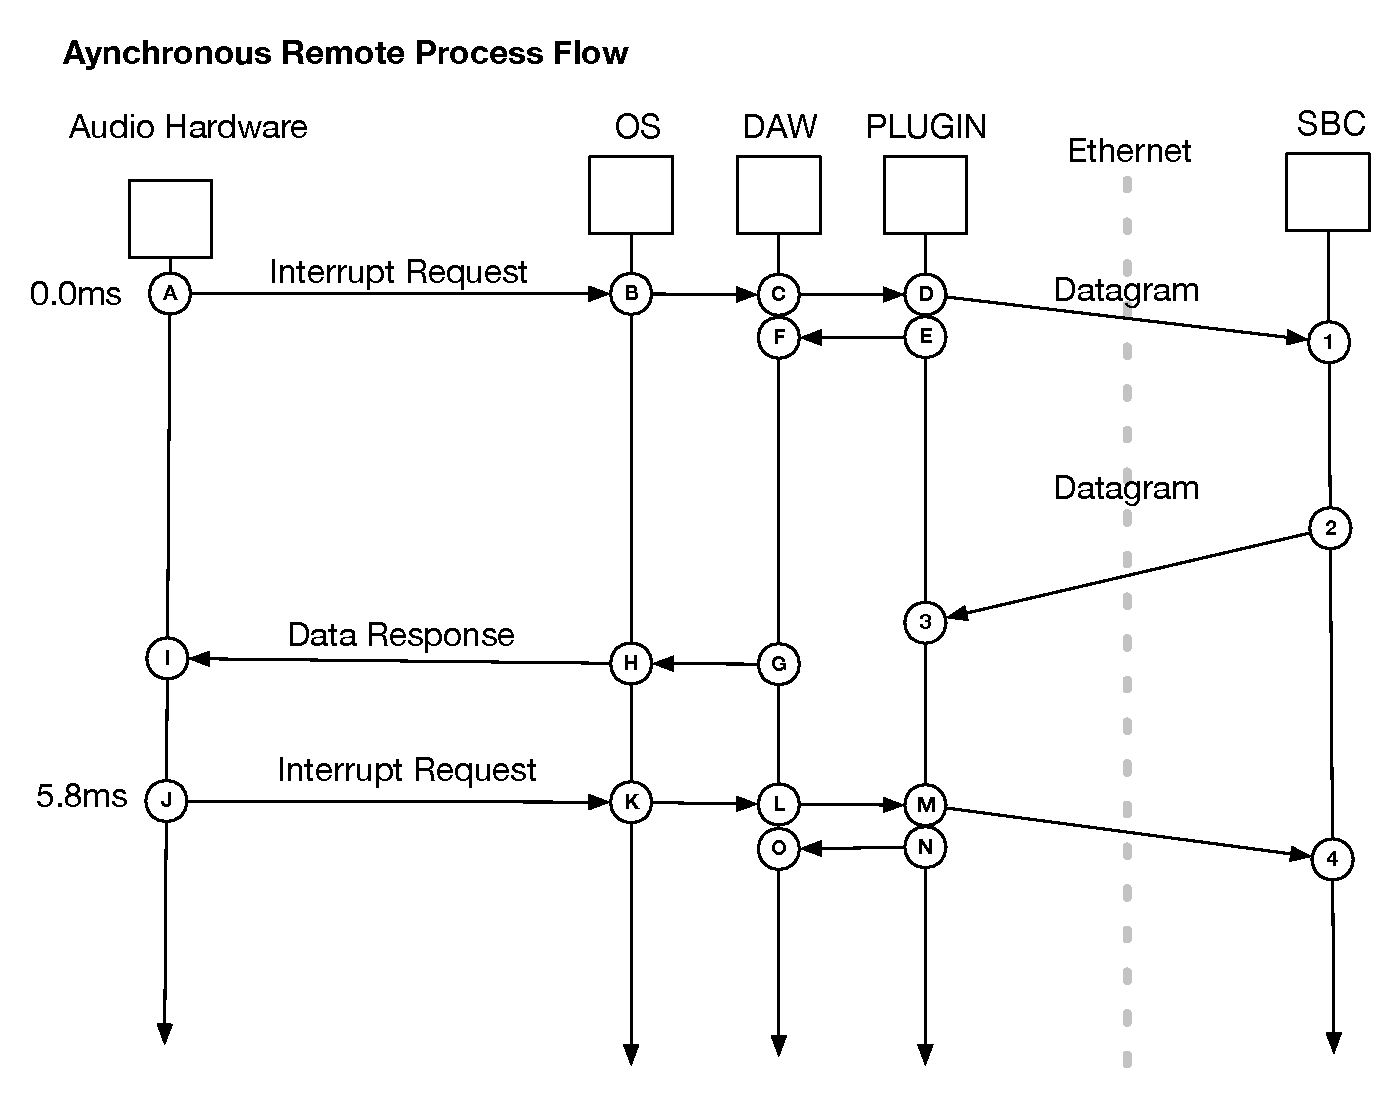
\includegraphics[width=\textwidth]{assets/conclusion/async_flow.pdf}
    \caption{Asynchronous Processing}
    \label{fig:async_remote}
\end{figure}

By the time the second cycle begins (J in figure~\ref{fig:async_remote}) processed data from the first cycle has returned. The time between events M and N is no longer proportional to the amount of time needed to actually process the data, only to the time it takes for sending and receiving. Table~\ref{tab:latency_async} shows the measured times.

\begin{table}[H]
\begin{center}
\begin{tabular}{ |p{1.4cm}||p{1.5cm}|p{1.7cm}|p{1.7cm}|p{1.6cm}|p{1.4cm}|  }
 \hline
 buffer size    & limit (ms)    & rtTime (ms)   & pTime (ms)    & tTime (ms) & \% of limit\\
 \hline
 64             & 1.451247      & 0.031683          & 0.015633          & 0.016050      & 2.18 \\
 96             & 2.176870      & 0.046585          & 0.016076          & 0.030509      & 2.14 \\
 128            & 2.902494      & 0.034745          & 0.016712          & 0.018032      & 1.19 \\
 192            & 4.353741      & 0.052279          & 0.018800          & 0.033478      & 1.20 \\
 256            & 5.804988      & 0.065752          & 0.019646          & 0.046105      & 1.13 \\
 512            & 11.60997      & 0.062939          & 0.019708          & 0.043230      & 0.54 \\
 \hline
\end{tabular}
\end{center}
\caption{Measured Times for Asynchronous Processing}
\label{tab:latency_async}
\end{table}

In the table above "rtTime" is no longer the actual round trip total processing time. Since data is already available at the time the interrupt request is triggered, the plugin can return it's data immediately. This comes at the cost of a delay equal to one interrupt cycle, but the user can set the audio system's buffer size low enough that this is well below the 10ms limit, without needing to use more than 1.2\% of the processing time available.

The asynchronous method brings a real benefit to distributed processing in terms of lighting the load on the CPU. The price of the benefit though is an increase in the latency of the plugin. The processed audio data is always one delayed by one buffer cycle. Another disadvantage is that if several distributed processors are chained in series, as is the case in the demo application, then the latency is cumulative. This results is a total latency that is the "buffer time" multiplied by the number of processors in the
plugin.

\subsection{Potential Optimisations }

There are two areas of the application where unnecessary operations are performed and could be optimized. The first is the deserializsation of data when it is returned from the SBC. If serveral processes in the Plugin are chained in series, then the returned DiauproMessage could be sent directly to the following process without unnecessarily deserialising and the reserialising the data in between steps. This would be a relatively simple optimization to implement.

The second optimisation is similar but more complicated to implement. In a chain to processes the data would not need to be returned to the master plugin between each step, instead it could be sent to the next node directly. If the next node is located on the same SBC device then an additional hop over ethernet could be skipped as well. In addition serialisation steps between nodes could also be skipped if the nodes performed the operations directly on the data in the DiauproMessage. For this the DiauproMessage would need to be extended to include routing information so that each node knows the next destination point.

Although more complex, the second optimization would have the added benefit that the latency would no longer be a multiple of the full cycle time between interrupt calls. The final data could be gathered after a single cycle.

\section{Summary}

The asynchronous implementation offers definite potential. The latency seems to be identical to commercial DSP based systems\cite{UAD2-review}. This is interesting as it suggests that the DSP and SBC based systems share some limitations and that these cannot simply be overcome by simply connecting a more powerful DSP or SBC device. The real barrier is getting the data back from the device as fast as possible without blocking the audio thread. If the audio thread is blocked for 10\% or 30\% of the time is irrelevant. By resigning to a method that skips a full cycle of the audio thread there is no need to block it. The difference in bandwidth between Thunderbolt, PCIe, or Gigabit-Ethernet connectivity only effects that number of plugins that can be run simultaneously but not the latency.

This is encouraging, especially considering the expandability of the SBC based system, and the compatibilty of the codebase. Two definite advantages that the SBC system has over DSP based systems.






